\section{Eficiencia energética}

\subsection{Levantamento das Cargas}
\label{levantamento-cargas}

Nesta seção cuidar-se-á em informar as características nominais das cargas que serão alimentadas pela energia elétrica gerada a partir da conversão da energia mecânica existente devido ao torque exercido no eixo da bicicleta pelo usuário do projeto. Assim, apresenta-se a Tabela xxx, a qual indica aquelas características daquelas cargas.
Sensores, celular (tensão nominal, fator de potência, potência requerida, corrente, potência aparente, faixa de tensão etc.).

\subsection{Fonte Geradora}
\label{fonte-geradora}

\subsubsection{Princípio de Funcionamento do Gerador Síncrono}
\label{gerador-sincrono}


Geradores síncronos são bastante utilizados em centrais elétricas, independente do seu tipo. Grande parcela da energia elétrica disponível mundialmente é gerada por esse tipo de geradores, que convertem energia mecânica em energia elétrica. Além da geração de energia elétrica para ser distribuída na rede elétrica, os geradores síncronos são usados na geração de energia de pequeno porte e autônoma, não conectada a rede elétrica, como é o caso do presente projeto. 
Uma máquina síncrona é constituída por enrolamentos de armadura alojados na parte estacionária, denominada estator. Esses enrolamentos são conhecidos como enrolamentos do estator. Além deles, há um segundo enrolamento denominado enrolamento de campo, no qual gera corrente contínua e é utilizado para produzir o principal fluxo de operação do gerador. Em um gerador síncrono, o enrolamento de campo encontra-se no rotor, de modo que a corrente em que a corrente deve ser fornecida através do contato rotativo mecânico.  Segundo Fitzgerald, é vantajoso em um gerador síncrono que o enrolamento de campo, único e de baixa potência, localize-se no rotor e o enrolamento de armadura, de potência elevada e geralmente polifásico, encontre-se no estator.
O princípio de funcionamento de um gerador síncrono assemelha-se ao de uma máquina de corrente contínua no que diz respeito à tensão induzida no condutor, gerada pelo movimento rotativo entre um condutor e um campo magnético. Em um gerador síncrono, os condutores são fixos na armadura e o campo magnético é forçado pela máquina primária a se mover. A máquina primária é acoplada ao rotor do gerador, onde se encontram os polos, submetendo-os a uma força que os fazem girar. Como consequência do movimento entre o condutor e o campo, surge a tensão nos terminais do gerador síncrono, na qual faz com que uma corrente circule pelo gerador e pela carga que será ligada no gerador. Com a tensão e a corrente induzida pelo movimento, a potência mecânica transferida pela máquina primária é então convertida em energia elétrica, levando em consideração as perdas existentes nesse fenômeno. O enrolamento de campo é alimentado por uma fonte de corrente contínua por meio de anéis deslizantes. A tensão gerada pelo gerador síncrono trata-se de uma tensão alternada senoidal, que pode ser monofásica ou trifásica.
Com o objetivo de aumentar a potência convertida, em um gerador síncrono não há apenas um condutor sendo movimentado no campo magnético, mas condutores ligados em série. Assim, a potência do gerador e o aproveitamento dos materiais são maiores. 

\subsubsection{Partes Construtivas do Gerador Síncrono}
\label{construtivas-gerador-sincrono}

O alternador é composto das seguintes partes: rotor, estator, carcaça, escova e anéis, ponte retificadora, ventilador, polias e parafusos. As principais partes construtivas de um alternador serão tratadas posteriormente no presente relatório.
Abaixo, na figura \ref{partes-alternador}, são mostradas essas partes que compõem um alternador de automóvel.


\begin{figure}[h]
	\centering
	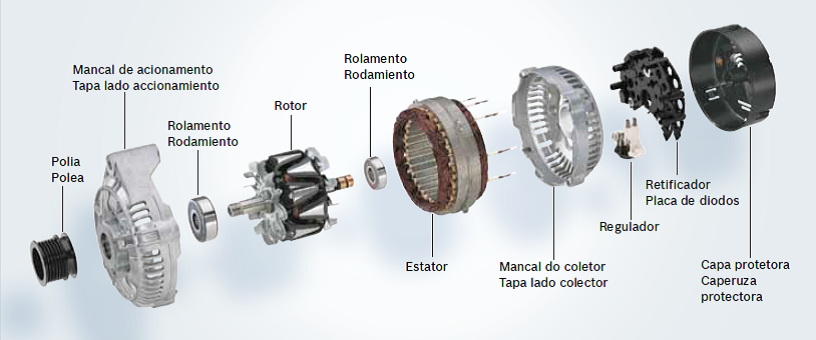
\includegraphics[scale= 0.8]		{figuras/partes_alternador.png}
	\caption{Partes que compõem um alternador}
	\label{partes-alternador}
\end{figure}

\begin{description}

\item [Rotor]
O rotor é trata-se da parte móvel no centro do alternador, constituído por um eixo de aço com uma bobina enrolada em seu interior, na qual a quantidade de fios de cobre da bobina varia de acordo com a capacidade e especificações de cada alternador. O rotor tem como principal função formar um campo magnético que tem como resultado a produção de corrente elétrica, onde os seus polos são alimentados com corrente contínua e geram o campo principal que induz tensão na armadura. A alimentação do enrolamento de excitação no alternador utilizado é feito através de anéis e escovas. 
Abaixo, na figura \ref{rotor-alternador}, pode ser visto o rotor do alternador utilizado no presente trabalho, representado pelo número 1.

\begin{figure}[h]
	\centering
	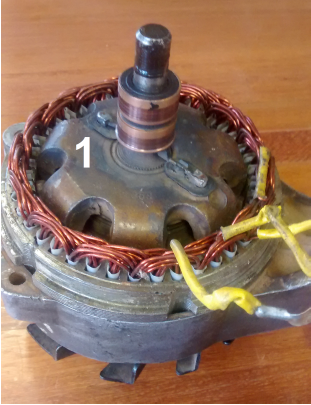
\includegraphics[scale=0.8] {figuras/rotor_alternador.png}
	\caption{Rotor do alternador}
	\label{rotor-alternador}
\end{figure}

\item [Estator]

O estator é formado por um conjunto de bobinas isoladas entre si e fixadas em um conjunto de laminas de aço. Essas lâminas têm características magnéticas de alta permeabilidade, proporcionando um caminho com pequena relutância para o fluxo, o que diminui o fluxo disperso e concentra o campo no entreferro. O uso de lâminas na construção do estator proporciona a diminuição das perdas provocadas por correntes parasitas em relação ao emprego de uma estrutura maciça. Essas lâminas também são tratas termicamente para diminuir o valor das perdas geradas por correntes induzidas.
Essa parte fundamental de um gerador síncrono tem como principal função a criação da corrente elétrica. Entretanto, para a geração de energia as boninas do estator requerem a produção de um campo magnético pelo rotor. A figura \ref{estator-alternador} apresenta o estator do alternador automotivo. 

\begin{figure}[h]
	\centering
	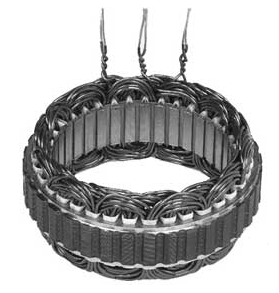
\includegraphics[scale=1]		{figuras/estator_alternador.png}
	\caption{Estator do alternador}
	\label{estator-alternador}
\end{figure}


\item [Regulador de Tensão]

O regulador de tensão do alternador é um dispositivo de proteção do mesmo, utilizado com o objetivo de proteger os equipamentos que usam a energia gerada pelo alternador, ou seja, as cargas conectadas a ele. O regulador protege as cargas por meio do controle da tensão produzida em qualquer regime de rotação do alternador, de modo a limitar a tensão para que não haja picos de corrente elétrica. Além disso, o regulador de tensão é usado com o objetivo de impedir que a bateria utilizada no projeto sofra sobrecarga. 

\item [Ponte Retificadora]
\end{description}

\subsubsection{Alternador Utilizado}

O gerador síncrono utilizado neste projeto trata-se de um alternador do automóvel Chevette com corrente nominal de 35 ampères e tensão de 14 volts. A figura \ref{alternador} apresentada abaixo mostra esse alternador.

\begin{figure}[h]
	\centering
	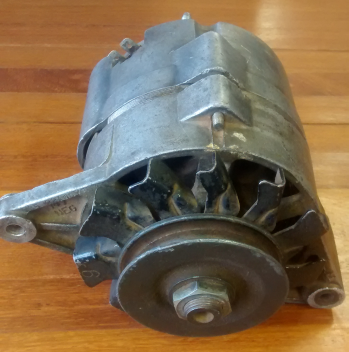
\includegraphics[scale=0.8]		{figuras/alternador.png}
	\caption{Alternador Utilizado}
	\label{alternador}
\end{figure}

\subsection{Cálculo da Corrente de Projeto Necessária}

A corrente de projeto necessária ao atendimento das cargas a ser alimentadas pelo circuito de distribuição da energia elétrica gerada deve ser determinada conforme a equação abaixo:

\begin{equation}
	\mathcal{I}_{proj} = \frac{{P}_{ativa}}{V \times FP}
\end{equation}

Onde:
\begin{description}

\item [Iproj] corrente de projeto em ampère

\item [Pativa] potência ativa total do circuito em watt

\item [V] tensão do circuito em volt

\item [FP] fator de potência total do circuito
\end{description}

Nesse sentido, com base nos dados informados na Tabela xx da seção xx deste relatório, tem-se que a corrente de projeto será igual a xx A.

	Entretanto, a corrente de projeto a ser adotada para o dimensionamento do circuito elétrico será tida como 35 ampères, devido ao fato deste valor ser a capacidade máxima de corrente elétrica que a fonte geradora aqui adotada poderá atingir.
	
	O fato de a corrente de projeto ter sido escolhida acima da necessidade real de nosso projeto é justificado pelo motivo da possibilidade futura de expansão das cargas alimentadas pelo circuito ora projetado, ocorrendo assim a desnecessidade de redimensionamento do sistema elétrico caso novas cargas fossem inseridas no mesmo.

\subsection{Dimensionamento dos Condutores}

O caminho percorrido pela energia elétrica ao longo de um circuito de distribuição deve ser projetado da maneira mais eficiente possível, desde a fonte geradora de corrente elétrica até as cargas terminais, uma vez que parcela daquela energia é dissipada sob a forma térmica devido à resistência elétrica que o fio condutor pelo qual a referida energia se movimenta exerce sobre o fluxo elétrico, restando, assim, prejudicada a eficiência final de distribuição da energia.

Nesse sentido, ao se projetar um circuito elétrico, deve-se procurar minimizar ao máximo possível as perdas de energia ao longo do mesmo e, agindo dessa maneira, terão sido, por conseqüência, observados aspectos ambientais e conservacionistas ligados ao desperdício de energia. Ademais, deve-se atentar que as perdas oriundas do calor gerado nos condutores de eletricidade reduzirão o nível da tensão disponível no circuito terminal.

Por isso, ao dimensionar os condutores pertinentes ao projeto elétrico ora em estudo, os aspectos acima mencionados foram levados em consideração, a fim de reduzir na prática as supracitadas perdas.
Seguindo esse raciocínio, a escolha dos condutores utilizados neste projeto foi realizada conforme especificações dispostas pela Associação Brasileira de Normas Técnicas (ABNT) na Norma Brasileira número 5410, de 2004 (NBR 5410:2004), cujo teor aborda critérios para o dimensionamento de instalações elétricas de baixa tensão. 
Desse modo, cuidou-se em dimensionar os referidos condutores de acordo com os critérios que visam auxiliar economia de energia, bem como economia de custos financeiros, a fim de atender às necessidades do nosso projeto.

Assim, conforme especificações técnicas daquela NBR, cuidou-se em identificar a “seção do condutor que reduza o custo da energia desperdiçada, sem incorrer em custos iniciais excessivos de compra e instalação de um cabo”, bem como dos dispositivos de proteção necessários, pautando-se pelos seguintes métodos:

\begin{itemize}
	\item Capacidade de condução de corrente
	\item Queda de tensão
	\item Seção mínima
	\item Proteção contra sobrecarga
	\item Proteção contra curto-circuito
	\item Choque elétrico
\end{itemize}

o final dos resultados, em princípio, cada um desses métodos poderá indicar uma seção diferente. Então, segundo a NBR, a seção a ser finalmente adotada consistirá na maior dentre todas as seções obtidas. Vejamos cada um desses métodos.

\subsubsection{Capacidade de Condução de Corrente (artigo 2)}

Segundo (Eletricidade Moderna), o dimensionamento do projeto elétrico seguindo todos os seis critérios mencionados na NBR em comento, têm sua relevância, embora seja compreensível que o critério da capacidade de condução de corrente apresente uma importância que parece ser superior às demais, surgindo como ponto de partida da escolha dos condutores apropriados.

Ainda no entendimento de (Eletricidade Moderna), o critério aqui discutido, de fato, logo após a determinação das cargas existentes no circuito, passando em seguida pelo cálculo da corrente de projeto (Iproj), tem como etapa seguinte, sendo considerada a primeira em relação ao dimensionamento dos componentes do circuito, a determinação da capacidade de condução de corrente do circuito, determinando assim a seção do condutor que proporcionará nas condições práticas de execução a capacidade de condução de corrente suficiente para a circulação de Iproj sem riscos.

Desse modo, em posse do valor de Iproj, bem como das características de constituição dos condutores, recorreu-se às tabelas que orientam o dimensionamento através do critério em análise, apurando-se a seção do condutor que atenda às necessidades do nosso circuito, vejamos.

Para o caso concreto,\textit{segundo as disposições da NBR}, quanto ao tipo de condutor empregado, ter-se-á condutor isolado (condutor metálico e isolação), sendo o material PVC (cloreto de polivinila). Isso é devido às características de trabalho listadas na Tabela \ref{nbr}, com informações extraídas da NBR.

\begin{table}[h]
\begin{tabular}{| c | p{3cm} | p{3cm} | p{3cm} |}
\hline
Tipo de isolação                & Temperatura máxima para serviço contínuo (condutor) & Temperatura limite de sobrecarga (condutor) & Temperatura limite de curto-circuito (condutor) \\ \hline
Cloreto de polivinila(PVC)      & 70                                                 & 100                                        & 160                                            \\ \hline
Borracha etileno-propileno(EPR) & 90                                                 & 130                                        & 250                                            \\ \hline
Polietileno-reticulado(XLPE)    & 90                                                 & 130                                        & 250                                           
\\ \hline
\end{tabular}
\label{nbr}
\caption{Características de condutores. Retirado do}
\end{table}

Cumpre informar que o motivo da escolha dos condutores com tipo de isolação PVC foi feita devido esse condutor suportar as condições de nosso projeto.

No que tange ao método de instalação a ser utilizado, levou-se em consideração o fato de que este influencia a capacidade de troca térmica entre os condutores e o ambiente circundante, alterando a capacidade de condução de corrente dos condutores. Por isso, através de visita à Tabela xxxx (abaixo) da NBR, foi definido qual método será o mais adequado às condições de nosso projeto, optando-se pelo método de instalação B1.

\begin{figure}[h]
	\centering
	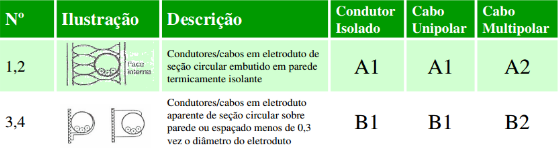
\includegraphics[scale=0.8]		{figuras/nbr.png}
	\caption{NBR - Definição do método}
	\label{alternador}
\end{figure}

Continuando, a NBR diz que a Iproj adotada deve ser corrigida por fatores de correção apropriados, os quais são: a) fatores de correção para temperaturas ambientes diferentes; b) correção de resistividade do solo; e c) fator de correção de agrupamento.

Uma vez que as condições de projeto do circuito em discussão não necessitam da utilização desses fatores, seguiu-se o dimensionamento com a Iproj anteriormente informada.

	O próximo passo foi determinar o esquema dos condutores, conforme opções listadas na Tabela \ref{metodo-definicao}. Optou-se pelo esquema monofásico a dois condutores.
	
\begin{table}[h]
\begin{tabular}{| l | l |}
\hline
Esquema de condutores vivos do circuito & Número de condutores carregados a ser adotado \\ \hline
Monofásico a dois condutores            & 2                                             \\ \hline
Monofásico a três condutores            & 2                                             \\ \hline
Duas fases sem neutro                   & 2                                             \\ \hline
Duas fases com neutro                   & 3                                             \\ \hline
Trifásico sem neutro                    & 3                                             \\ \hline
Trifásico com neutro                    & 3 ou 4
\\ \hline
\end{tabular}
\label{metodo-definicao}
\end{table}

Após a definição dessas características/parâmetros, o próximo passo foi consultar a Tabela xxx da NBR para efetivar a escolha da seção dos condutores apropriados às condições de projeto, consoante o critério aqui descrito. Portanto, chegou-se à escolha do condutor de seção xxx.

\subsubsection{Queda de Tensão (disposições da UFJF)}

A importância da aplicação desse critério consiste no fato de que as cargas consumidoras de energia elétrica foram projetadas para trabalharem com determinado valor de tensão, aceitando, apenas, reduzida tolerância de não-conformidade com o valor de tensão nominal para o qual a carga foi projetada.
Assim, ao utilizar esse critério, foi levada em consideração a possibilidade dos efeitos anormais que a queda de tensão poderá acarretar às cargas.
 Segundo esse critério, “à medida que a distância entre o medidor de energia e a potência da carga aumenta a queda de tensão ao longo do condutor também aumenta”. 
Por isso, baseando-se nesse critério, e com auxílio das características dos condutores adotados neste projeto (PVC, eletroduto não magnético e método de referência B1), somado ao fato de que a NBR informa que em baixa tensão, a queda de tensão nos circuitos terminais não pode ser superior a 4\%, calculou-se a seção dos condutores, veja.

\begin{description}

	\item Cálculo da Queda de Tensão
	%pegar as equaçoes
	
	Com esse resultado, visitou-se a Tabela xxx da fabricante Pirelli e constatou-se que para as condições do nosso projeto, a seção do condutor deve ser 6 mm\textsuperscript{2}.
(Lembrar que deve ser atentado ao cálculo da queda de tensão por trecho)

\begin{equation}
	\Delta V = \Delta V_{\frac{V}{A \times km}} \times I_{proj} \times L
\end{equation}
\begin{equation}
	\Delta V_{\frac{V}{A \times km}} = \frac{\Delta V} {I_{proj} \times L}
\end{equation}
\begin{equation}
	\Delta V_{\frac{V}{A \times km}} = \frac{0,04 \times 14}{35 \times 0,002}
\end{equation}
\begin{equation}
	\Delta V_{\frac{V}{A \times km}} = 8 \times \frac{V}{A \times km}
\end{equation}

\end{description}

\subsubsection{Seção Mínima}

As seções mínimas admitidas em qualquer instalação de baixa instalação estão indicadas na Tabela \ref{secoes-minimas}, item xx da referida Norma. Nesse quesito, traduz-se a tabela, abaixo:

\begin{table}[h]
\begin{tabular}{ |l | p{7cm} | p{5cm} |}
\hline
Instalação                          & Número de condutores carregados a ser adotado           & Seção Mínima para condutores de cobre (mm\textsuperscript{2}) \\ \hline
\multirow{3}{*}{Fixas em geral}     & Circuitos de Iluminação                                 & 1,5                                        \\ \cline{2-3}
                                    & Circuitos de Força                                      & 2,5                                        \\ \cline{2-3}
                                    & Circuitos de sinalização e controle                     & 0,5                                        \\ \hline
\multirow{3}{*}{Ligações flexíveis} & Para um equipamento específico                          & Como especificado na norma do equipamento  \\ \cline{2-3}
                                    & Para qualquer outra aplicação                           & 0,75                                       \\ \cline{2-3} 
                                    & Circuitos a extrabaixa tensão para aplicaçòes especiais &                                           
\\ \hline

\end{tabular}
\label{secoes-minimas}
\caption{Seções Mínimas}
\end{table}

Assim, dentro desse quesito, adotou-se que as ligações de nosso circuito serão do tipo flexíveis, sendo a utilização consistente com circuitos de extra-baixa tensão para aplicações especiais. 

Por isso, levando-se em consideração a Tabela acima, a seção indicada é 0,75 mm\textsuperscript{2} para os condutores de cobre.

\subsubsection{Outros}

Porém, “como isto significa aumentar o custo do cabo, tende-se a anular a economia conseguida pela melhoria da eficiência na distribuição, sendo que é necessário encontrar-se então um compromisso entre estas duas variáveis”.

Por isso, visando economia de energia e uma distribuição de alta eficiência, procurou-se escolher os condutores deste projeto portando-se pela NBR em comento.

\subsection{Dimensionamento dos Dispositivos de Proteção do Circuito}

A proteção é uma ação automática provocada por dispositivos sensíveis a determinadas condições anormais, no sentido de evitar ou limitar danos a um sistema ou equipamento, a proteção também pode ser entendida como uma manobra automática.

A escolha, aplicação e a coordenação seletiva adequadas ao conjunto de componentes que constituem a proteção de um sistema é um dos aspectos mais importantes da instalação elétrica industrial. A função da proteção justamente minimizar os danos ao sistema e seus componentes, sempre que ocorrer uma falha no equipamento, no sistema elétrico ou falha humana.

Os dispositivos de proteção contra correntes de curto-circuito, como: disjuntores e fusíveis. E os dispositivos de proteção contra correntes de sobrecarga, como os relés bimetálicos.